% !TEX root = ../main.tex

A jelen fejezet az YJMob100K adathalmaz rácskoordinátáinak georeferálását és térképes megjelenítését mutatja be. A vizualizáció OpenStreetMap alaptérképre vetítve, pyproj-alapú koordináta-transzformációval készült.

\subsection{Georeferálási módszertan}

Az YJMob100K adathalmaz nem hozza nyilvánosságra a mérési helyszínt; az adatrekordok koordinátái 1--200 közötti rácsindexek, nem geodéziai koordináták. A rács valós térbeli elhelyezkedéséhez a \textit{reverse-engineering-YJMob100K-grid} projekt \cite{pinter2024revealing} eredményeit alkalmaztam, amely sablonillesztéssel azonosította a megfigyelési területet Nagoya városával (Aichi prefektúra, Japán).

A meghatározott koordináta-rendszer az EPSG:2449 (Japan Plane Rectangular CS~VII), amelynek origója 36°~északi szélesség és 137°~35'~keleti hosszúság. Az adatkészletben az $x$ tengelyindex az észak--déli (\textit{northing}), az $y$ index a kelet--nyugati (\textit{easting}) irányba növekszik (lásd 5.~fejezet).

Ellentétben a névleges 500~m-es rácsmérethivatkozással, a cellák nem négyzetesek: az easting irányú méret $5000 / 11 \approx 454{,}5$~m, a northing irányú méret $5000 / 9 \approx 555{,}6$~m. Az 5.\ fejezetben jelzett aszimmetria elkerülésére a \texttt{features.py} mindkét értéket explicit módon alkalmazza (ld.\ 7.\ fejezet).

A rács sarokpontja (az $(1, 1)$ cella bal alsó sarka) EPSG:2449-ben: easting $= {-60\,682}$~m, northing $= {-166\,667}$~m. Az ebből levezetett teljes kiterjedés: $\approx 91$~km (kelet--nyugat) × $\approx 111$~km (észak--dél).

\subsection{Megvalósítás}

A georeferálást a \texttt{geo.py} modul végzi. A pyproj könyvtár \texttt{Transformer} osztálya egyszer inicializálja az EPSG:2449 $\rightarrow$ WGS84 transzformációt, amelyet ezután vektorizáltan alkalmazom a teljes rácsra:

\begin{lstlisting}[language=Python, caption={Cellaindex WGS84-koordinátává alakítása.}, label={lst:geotransform}, basicstyle=\small\ttfamily, breaklines=true, frame=single]
from pyproj import Transformer
_to_wgs84 = Transformer.from_crs(
    "EPSG:2449", "EPSG:4326", always_xy=True)

def grid_to_lonlat(x, y):
    easting  = EASTING_MIN  + (y - 0.5) * CELL_WIDTH_M
    northing = NORTHING_MIN + (x - 0.5) * CELL_HEIGHT_M
    return _to_wgs84.transform(easting, northing)
\end{lstlisting}

A \texttt{make\_polygon\_gdf} függvény az összes rácscella poligonját Shapely \texttt{box} objektumként állítja elő, amelyeket GeoPandas GeoDataFrame-be gyűjt. Az alaptérkép megjelenítéséhez szükséges Web Mercator (EPSG:3857) vetületre a \texttt{.to\_crs()} metódus végzi az átváltást, a contextily könyvtár pedig a megfelelő OpenStreetMap csemperéteget tölti le és illeszti a kivetítési körzethez.

\subsection{Térképes vizualizációk}

A négy fő tematikus térképet egyetlen kompakt panelként mutatom be (\autoref{fig:gis_panel}): (a)~ping-aktivitás logaritmikus skálán~-- a belvárosban és a közlekedési csomópontok körül sűrűsödő ping-szám jól kirajzolja Nagoya körvonalát; (b)~az alapidőszak és a vészhelyzet ($d \geq 60$) közötti aktivitás-változás cellaszinten~-- területileg heterogén kép, a belvárosban csökkenés, az ipari körzetekben stagnálás (megerősíti a 9.~fejezet POI-zóna megfigyelését); (c)~POI-zónatérkép a 85 kategória 9 összevont típusra szervezve~-- a szolgáltatási (8\,664 cella) és ipari (4\,386 cella) zónák dominálnak, parkolói besorolásban mindössze 19 cella van; (d)~anomáliadetekció térbeli vetítése~-- az anomális felhasználó--nap arányok a város perifériáján és a fő kijáratoknál sűrűsödnek, összhangban a 9.~fejezet kontrakciós-paradoxon hipotézisével.

\begin{figure}[H]
\centering
\begin{tabular}{cc}
\includegraphics[width=0.46\textwidth]{img/gis_01_activity_map.png} &
\includegraphics[width=0.46\textwidth]{img/gis_02_baseline_vs_emergency.png} \\
(a) Aktivitás-sűrűség (log) & (b) Alap-vs.\ vészhelyzeti változás \\[0.6em]
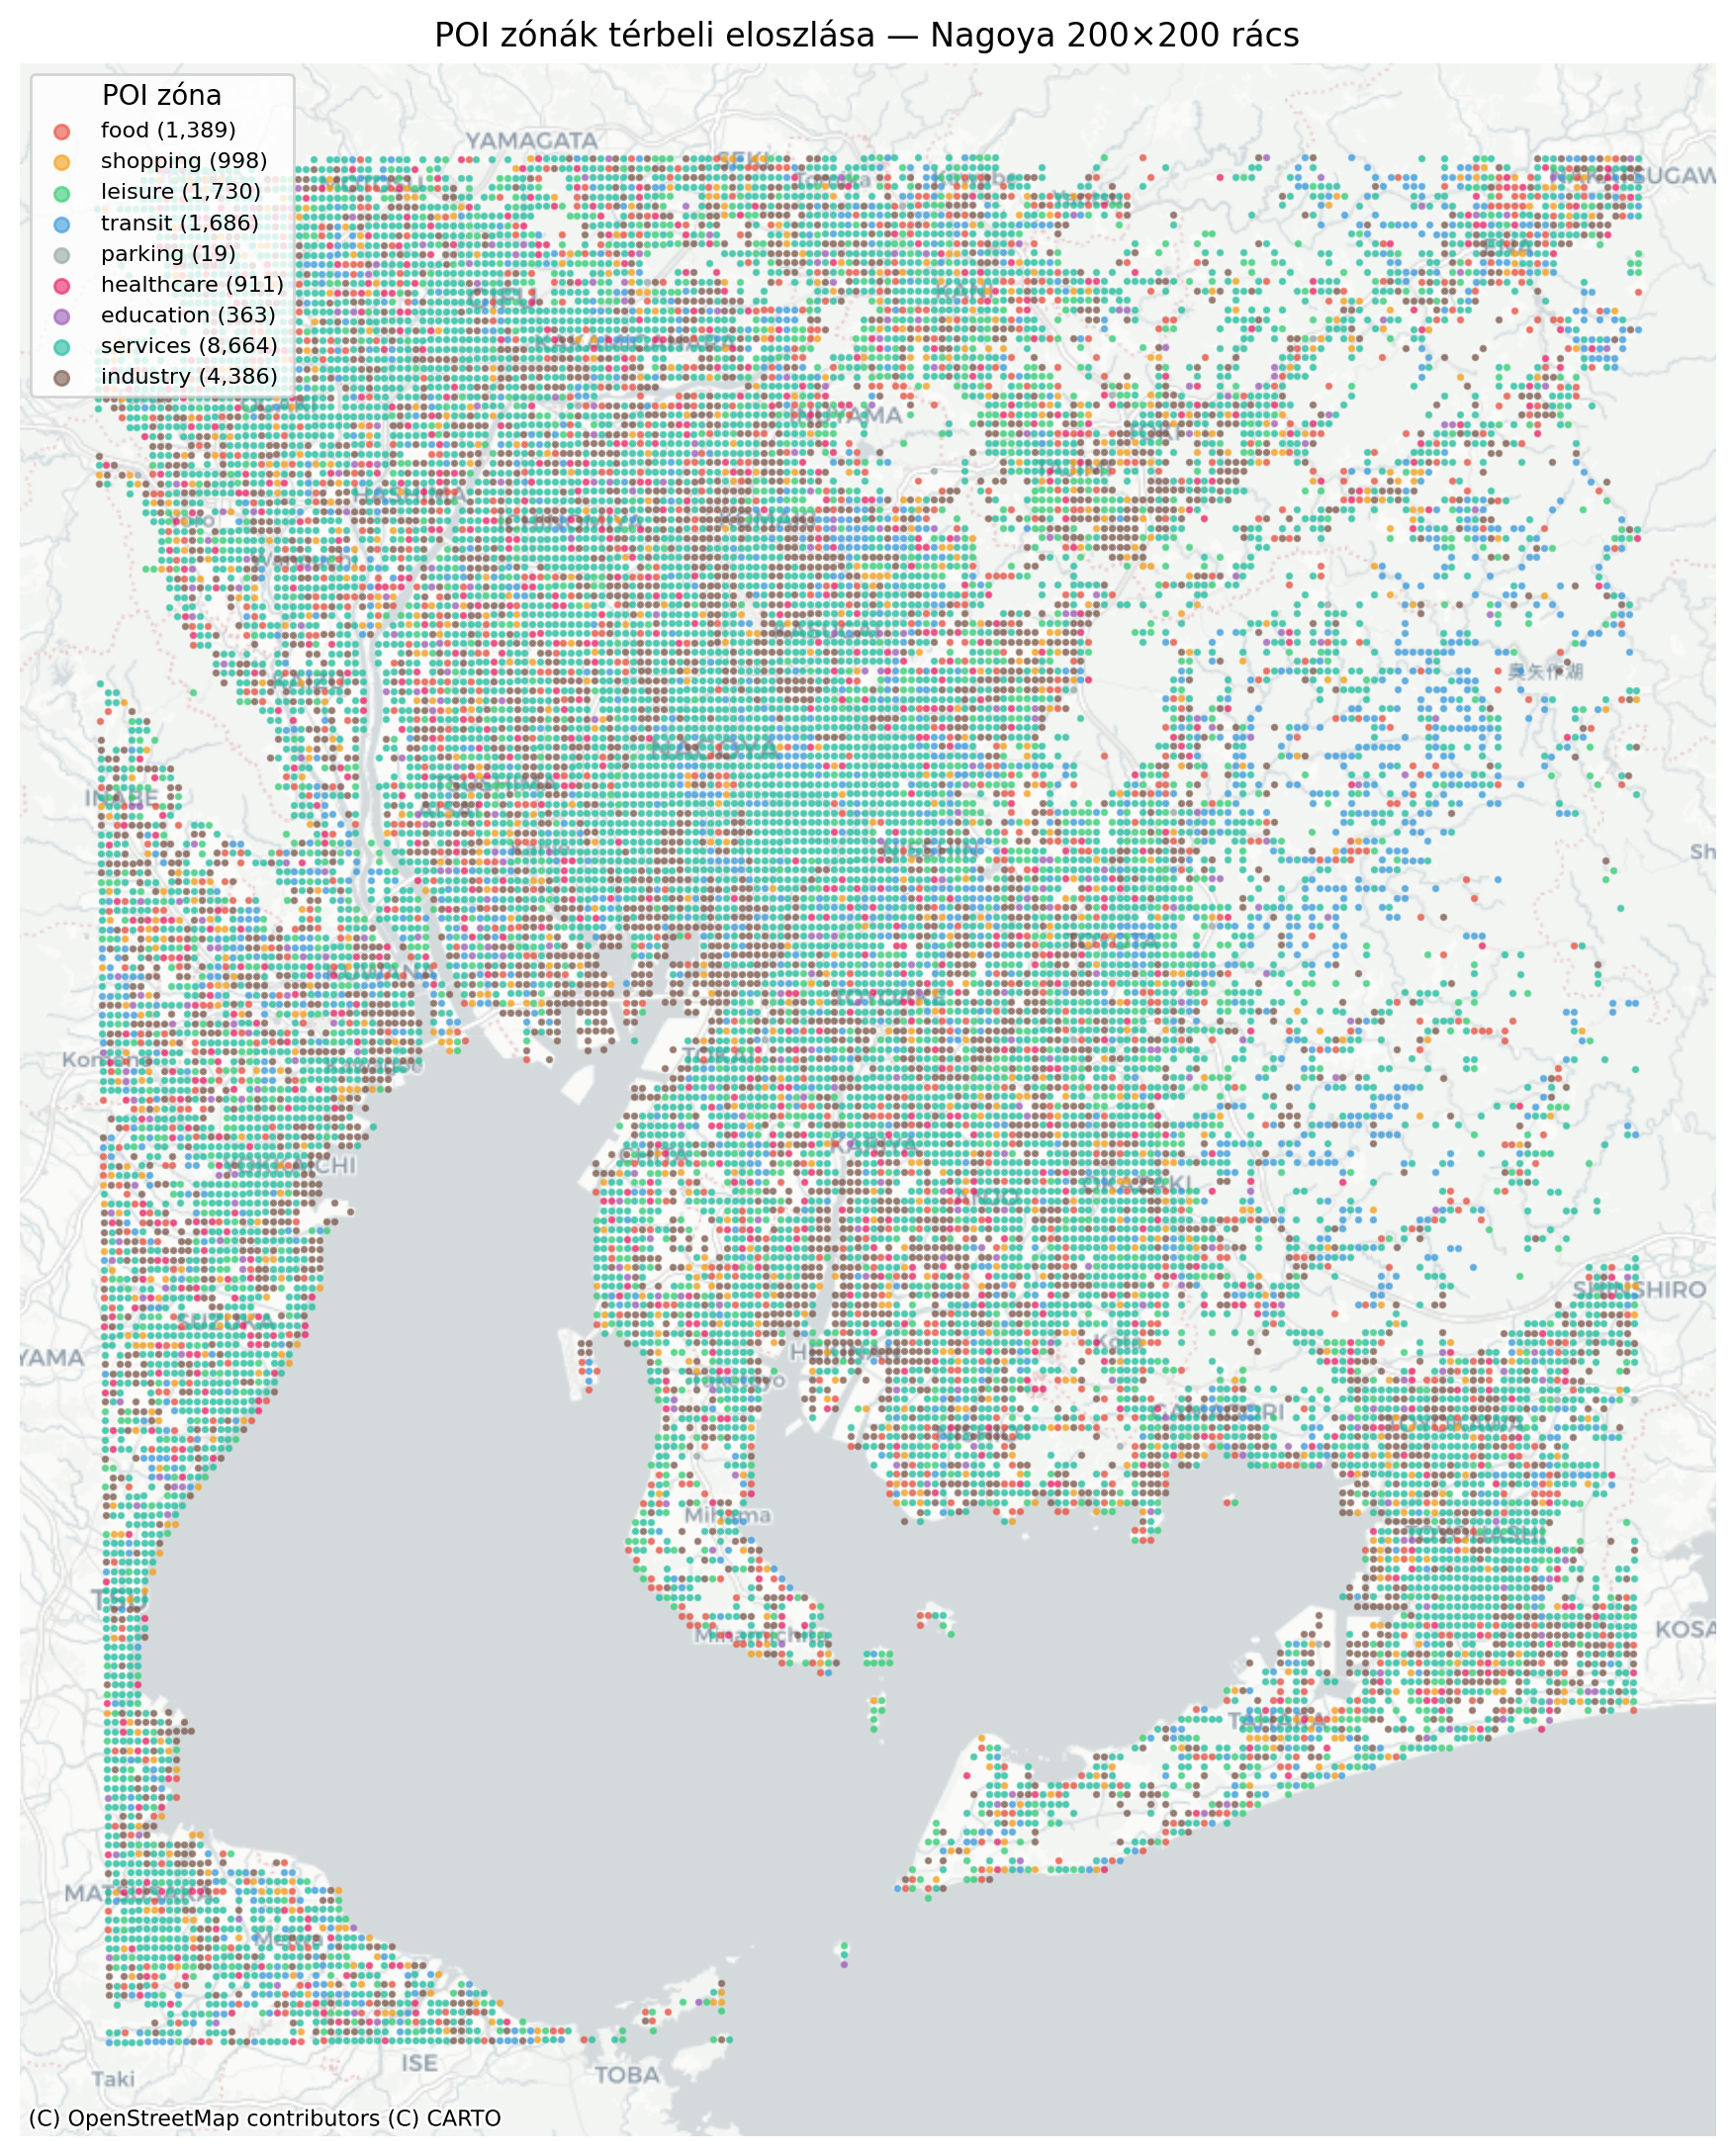
\includegraphics[width=0.46\textwidth]{img/gis_03_poi_zones.png} &
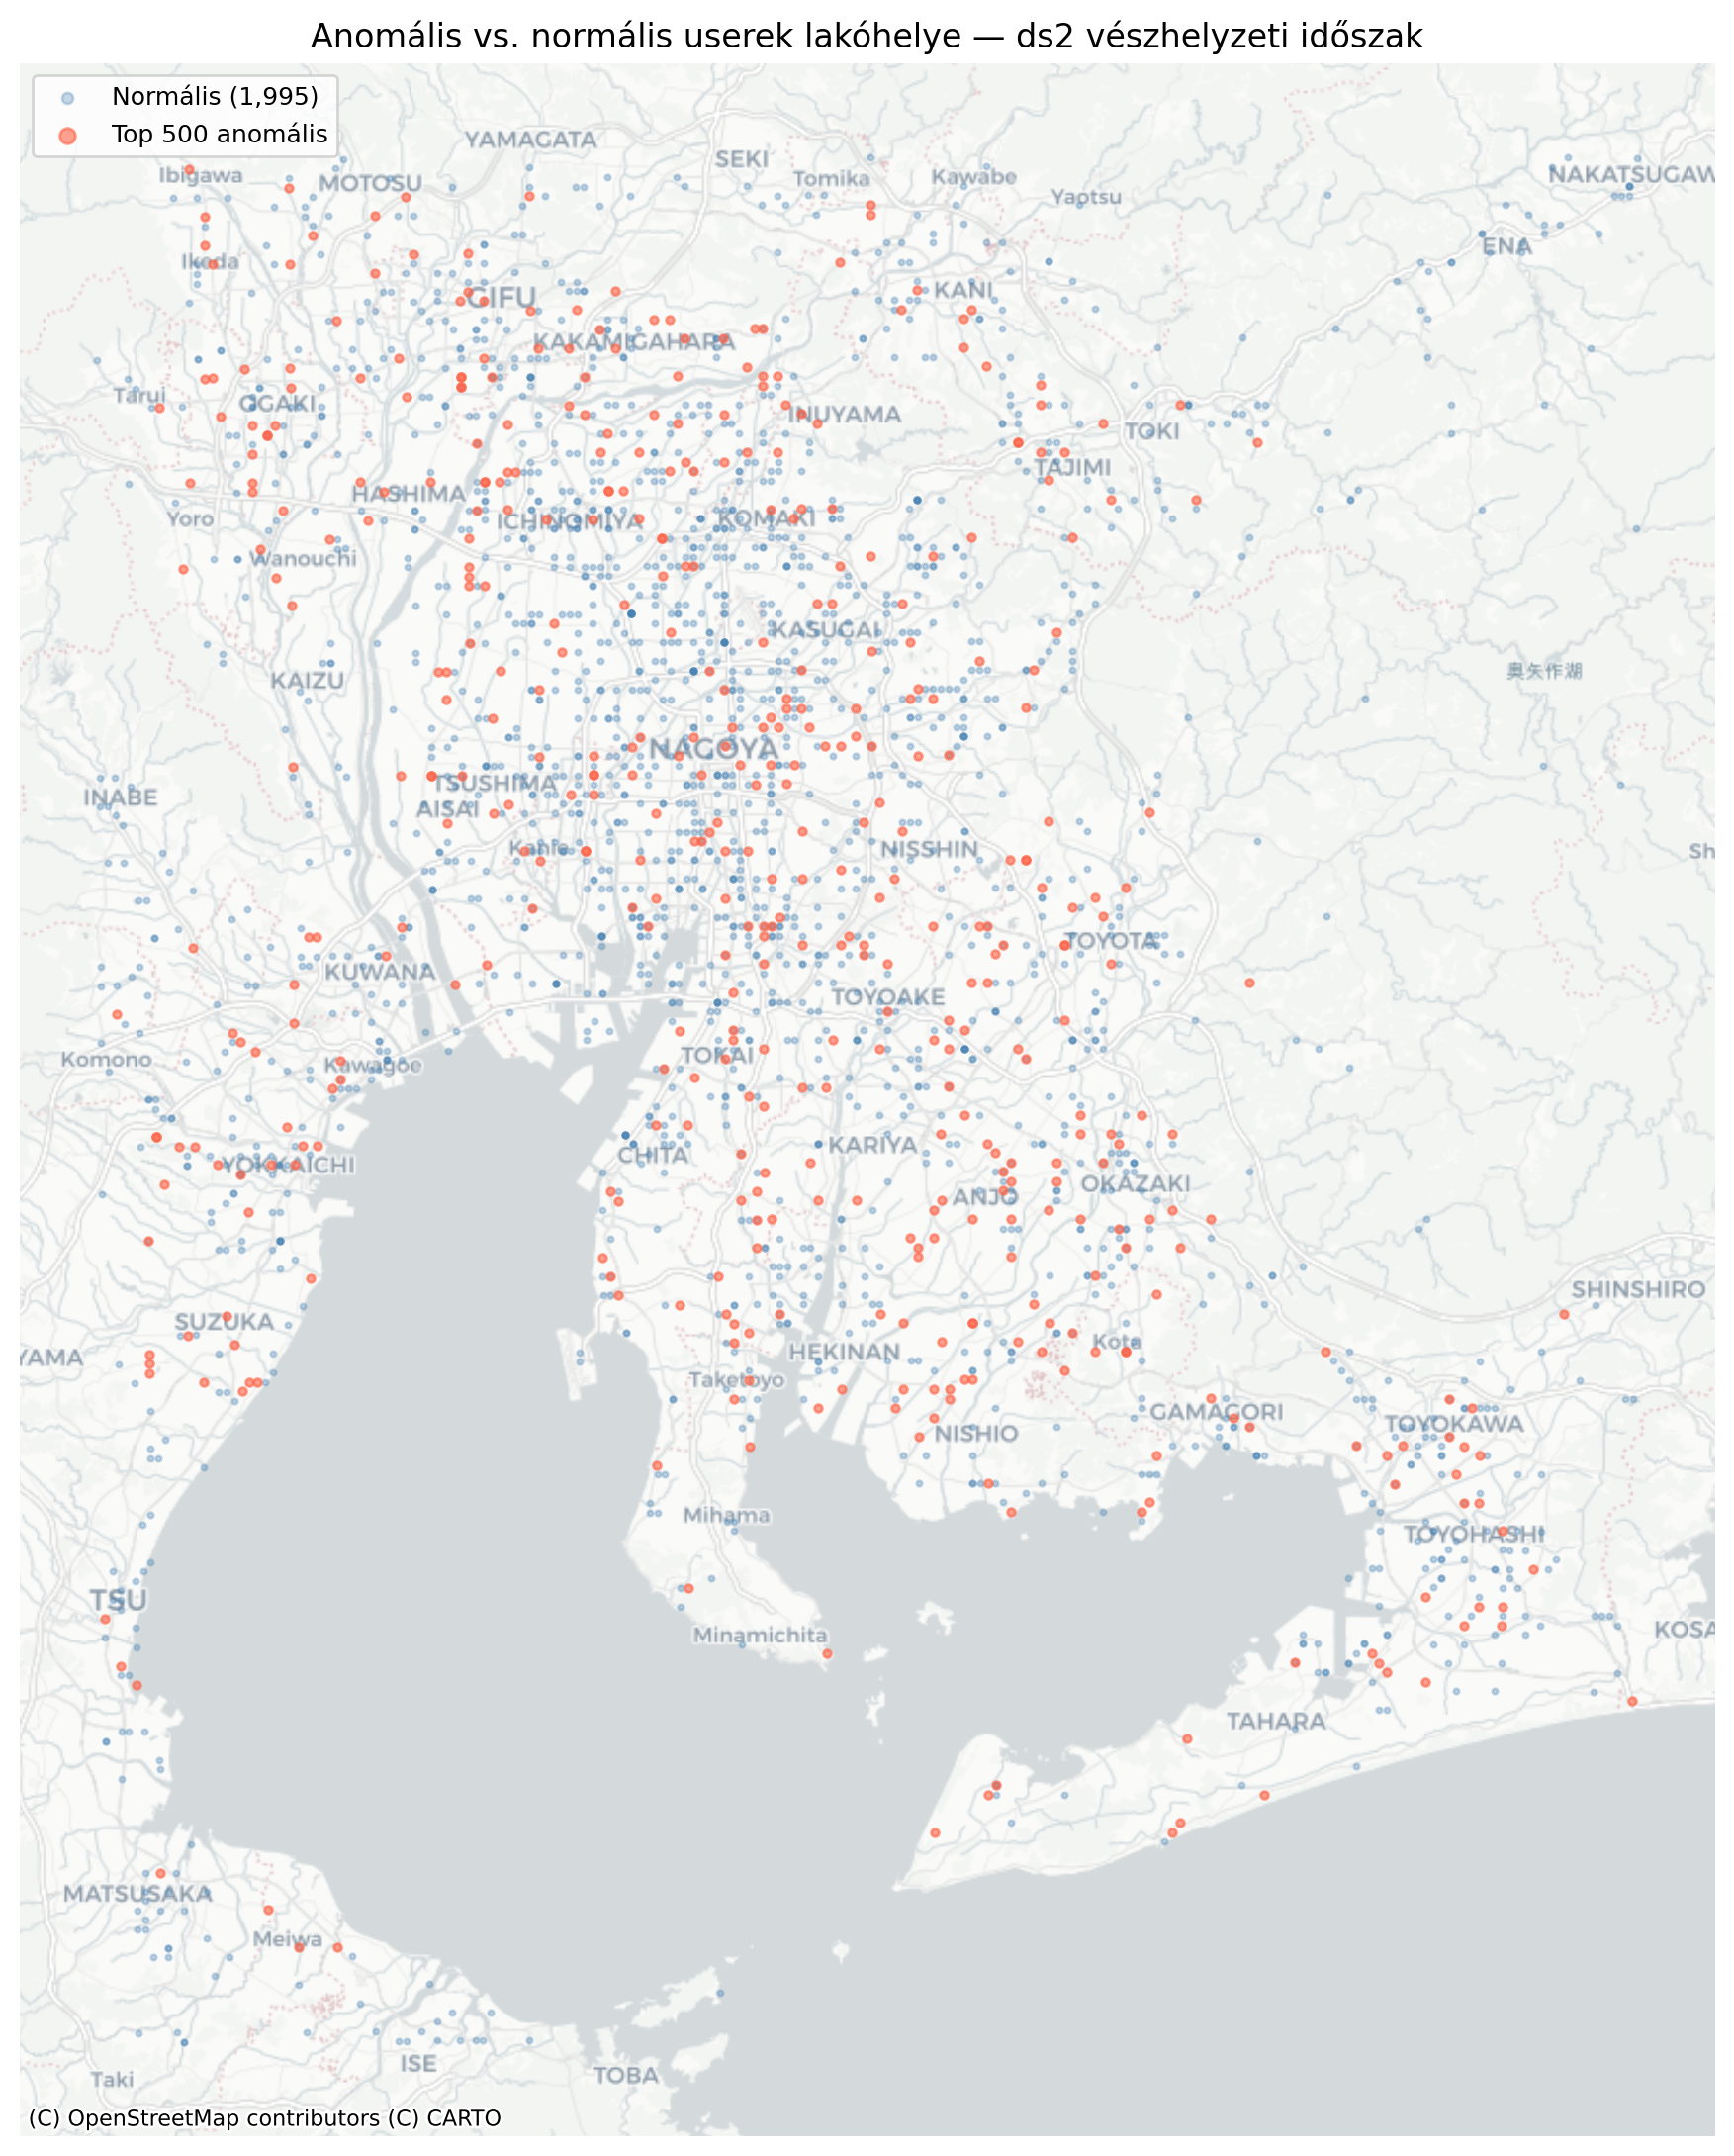
\includegraphics[width=0.46\textwidth]{img/gis_05_anomaly_map.png} \\
(c) POI-zónatérkép & (d) Anomáliák térbeli eloszlása \\
\end{tabular}
\caption{A négy tematikus GIS térkép Nagoya rácsán, OpenStreetMap \copyright{} alaptérképen. Saját szerkesztés.}
\label{fig:gis_panel}
\end{figure}
